\documentclass[12pt,a4paper]{article}
\usepackage[utf8]{inputenc}
\usepackage[english]{babel}
\usepackage{csquotes}
\usepackage{amsmath, amsfonts, amssymb, array}
\usepackage{graphicx, subcaption}
\usepackage{setspace}
\usepackage{multicol}
\usepackage{parskip}
\setlength{\parindent}{4em}
\usepackage{fancyhdr}
\usepackage{hyperref}
\usepackage{pgfplots}
\pgfplotsset{compat=newest}% use newest version
\usepackage{tikz, tikz-3dplot,  circuitikz}
\usepackage{xcolor}
\usepackage{sectsty}
\usepackage{xstring}
\usepackage{caption}
\usepackage{listings}
\usepackage{biblatex}
\addbibresource{citations.bib}
\usepackage{dirtytalk}
\usepackage{units}

\definecolor{blue2}{HTML}{206B99}



\usetikzlibrary{calc}
\begin{document}



\begin{figure}  \label{fig:overfitting}
    \centering
    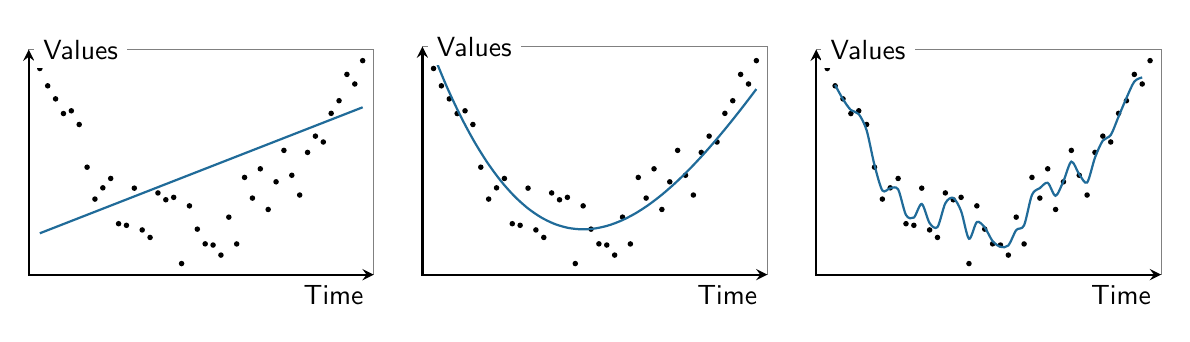
\begin{tikzpicture}[font=\sffamily,
    declare function={f(\x)=0.5*pow(abs(\x-2),2)-0.06*pow(\x-2,3);}]
     \foreach \Z in {1,...,42}
     {\pgfmathsetmacro{\X}{\Z/10}
     \pgfmathsetmacro{\Y}{f(\X)+0.9*rnd}
     \ifnum\Z=1
      \xdef\LstOne{(\X,\Y)}
      \xdef\LstTwo{"(\X,\Y)"}
     \else
      \xdef\LstOne{\LstOne (\X,\Y)}
      \xdef\LstTwo{\LstTwo,"(\X,\Y)"}
     \fi}
    %  \begin{scope}[local bounding box=over0]
    %  \foreach \Z in {1,...,42}
    %  {\pgfmathsetmacro{\Coor}{{\LstTwo}[\Z-1]}
    %  \fill \Coor circle[radius=1pt];
    %  }
    %  \draw plot[smooth] coordinates \LstOne;
    %  \end{scope}
     \begin{scope}[local bounding box=over,xshift=-5cm]
     \foreach \Z in {1,...,40}
     {\pgfmathsetmacro{\Last}{{\LstTwo}[\Z-1]}
     \pgfmathsetmacro{\Current}{{\LstTwo}[\Z]}
     \pgfmathsetmacro{\Next}{{\LstTwo}[\Z+1]}
     %\typeout{\Last,\Current,\Next}
      \edef\temp{\noexpand\path ($0.6*\Current+0.2*\Last+0.2*\Next$)   coordinate 
      (p\Z);}
      \temp
      \ifnum\Z=1
      \xdef\LstThree{(p\Z)}
      \else
      \xdef\LstThree{\LstThree (p\Z)}
      \fi
      }
     \foreach \Z in {1,...,42}
     {\pgfmathsetmacro{\Coor}{{\LstTwo}[\Z-1]}
     \fill \Coor circle[radius=1pt];
     }
     \draw[thick,blue2] plot[smooth] coordinates \LstThree;
%     \caption{Underfitting}
     \end{scope}
     %
     \begin{scope}[local bounding box=good,xshift=-10cm]
     \foreach \Z in {1,...,42}
     {\pgfmathsetmacro{\Coor}{{\LstTwo}[\Z-1]}
     \fill \Coor circle[radius=1pt];
     }
     \draw[thick,blue2] plot[smooth,domain=0.1:4.2,variable=\x] (\x,{f(\x)+0.45});
%     \caption{Good fit}
     \end{scope}
     %
     \begin{scope}[local bounding box=under,xshift=-15cm]
     \foreach \Z in {1,...,42}
     {\pgfmathsetmacro{\Coor}{{\LstTwo}[\Z-1]}
     \fill \Coor circle[radius=1pt];
     }
     \draw[thick,blue2] (0.1,0.4) -- (4.2,2);
%     \caption{Overfitting}
     \end{scope}
     %
     \foreach \X in {over,good,under}
     {\draw[gray,thin] ([xshift=-3pt,yshift=3pt]\X.north west) rectangle 
     ([xshift=3pt,yshift=-3pt]\X.south east);
     \draw[stealth-stealth,thick] ([xshift=-3pt,yshift=3pt]\X.north west) node[right=1.5pt,fill=white]{Values} 
     |- ([xshift=3pt,yshift=-3pt]\X.south east) node[below left]{Time};}
\end{tikzpicture}

\caption{lets see}
\end{figure}
\end{document}



%%%%%%%% TRYING  TO  FIX SUBCAPS %%%%%%%%%


\begin{figure}  \label{fig:overfitting}
    \centering
    \begin{subfigure}
        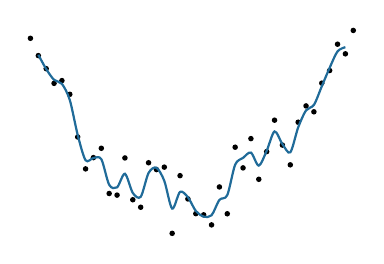
\begin{tikzpicture}[font=\sffamily,
        declare function={f(\x)=0.5*pow(abs(\x-2),2)-0.06*pow(\x-2,3);}]
         \foreach \Z in {1,...,42}
         {\pgfmathsetmacro{\X}{\Z/10}
         \pgfmathsetmacro{\Y}{f(\X)+0.9*rnd}
         \ifnum\Z=1
          \xdef\LstOne{(\X,\Y)}
          \xdef\LstTwo{"(\X,\Y)"}
         \else
          \xdef\LstOne{\LstOne (\X,\Y)}
          \xdef\LstTwo{\LstTwo,"(\X,\Y)"}
         \fi}
        %  \begin{scope}[local bounding box=over0]
        %  \foreach \Z in {1,...,42}
        %  {\pgfmathsetmacro{\Coor}{{\LstTwo}[\Z-1]}
        %  \fill \Coor circle[radius=1pt];
        %  }
        %  \draw plot[smooth] coordinates \LstOne;
        %  \end{scope}
         \begin{scope}[local bounding box=over,xshift=-5cm]
         \foreach \Z in {1,...,40}
         {\pgfmathsetmacro{\Last}{{\LstTwo}[\Z-1]}
         \pgfmathsetmacro{\Current}{{\LstTwo}[\Z]}
         \pgfmathsetmacro{\Next}{{\LstTwo}[\Z+1]}
         %\typeout{\Last,\Current,\Next}
          \edef\temp{\noexpand\path ($0.6*\Current+0.2*\Last+0.2*\Next$)   coordinate 
          (p\Z);}
          \temp
          \ifnum\Z=1
          \xdef\LstThree{(p\Z)}
          \else
          \xdef\LstThree{\LstThree (p\Z)}
          \fi
          }
         \foreach \Z in {1,...,42}
         {\pgfmathsetmacro{\Coor}{{\LstTwo}[\Z-1]}
         \fill \Coor circle[radius=1pt];
         }
         \draw[thick,blue2] plot[smooth] coordinates \LstThree;
         \end{scope}
         \end{tikzpicture}
     \caption{Underfitting}
     \end{subfigure}
     %
     \begin{subfigure}
        \begin{tikzpicture}[font=\sffamily,
         \begin{scope}[local bounding box=good,xshift=-10cm]
         \foreach \Z in {1,...,42}
         {\pgfmathsetmacro{\Coor}{{\LstTwo}[\Z-1]}
         \fill \Coor circle[radius=1pt];
         }
         \draw[thick,blue2] plot[smooth,domain=0.1:4.2,variable=\x] (\x,{f(\x)+0.45});
    
         \end{scope}
         \end{tikzpicture}
     \caption{Good fit}
     \end{subfigure}
     %   
     \begin{subfigure}
         \begin{tikzpicture}[font=\sffamily,
        
         \begin{scope}[local bounding box=under,xshift=-15cm]
         \foreach \Z in {1,...,42}
         {\pgfmathsetmacro{\Coor}{{\LstTwo}[\Z-1]}
         \fill \Coor circle[radius=1pt];
         }
         \draw[thick,blue2] (0.1,0.4) -- (4.2,2);

         \end{scope}
         \end{tikzpicture}
    \caption{Overfitting}
    \end{subfigure}

     %
     \foreach \X in {over,good,under}
     {\draw[gray,thin] ([xshift=-3pt,yshift=3pt]\X.north west) rectangle 
     ([xshift=3pt,yshift=-3pt]\X.south east);
     \draw[stealth-stealth,thick] ([xshift=-3pt,yshift=3pt]\X.north west) node[right=1.5pt,fill=white]{Values} 
     |- ([xshift=3pt,yshift=-3pt]\X.south east) node[below left]{Time};}
        
    
\caption{lets see}
\end{figure}
\end{document}